%------------------------------------------%
%
% Cannabis Data Science #61
%
% Date: 4/13/2022
%
%------------------------------------------%
\documentclass[xcolor={dvipsnames}]{beamer}
\hypersetup{pdfpagemode = FullScreen}
\mode<presentation>{
  \usetheme{Boadilla}
  \usecolortheme{orchid}
  \usefonttheme{default}
  \setbeamertemplate{navigation symbols}{}
  \setbeamertemplate{caption}[numbered]
}
\setbeamersize{
  text margin left = 0.5in,
  text margin right = 0.5in
}

%------------------------------------------%
% Title
%------------------------------------------%
\title[\textbf{Cannabis Data Science \#61}]{}
\author{Cannlytics}
\institute[]{\Large Cannabis Data Science \#61}
\date{April \nth{13}, 2022}

%------------------------------------------%
% Packages
%------------------------------------------%
\usepackage[english]{babel}
\usepackage[utf8x]{inputenc}
\usepackage{tikz} % For styling.
\usepackage{xparse}

%------------------------------------------%
% Colors
%------------------------------------------%
\definecolor{Green}{RGB}{34, 153, 84}
\definecolor{LightGreen}{RGB}{218, 247, 166}
\definecolor{DarkGreen}{RGB}{2, 48, 32}
\definecolor{Orange}{RGB}{255, 87, 51}
\definecolor{DarkOrange}{RGB}{199, 0, 57}
\definecolor{Yellow}{RGB}{255, 195, 0}

%------------------------------------------%
% Theme
%------------------------------------------%
\setbeamercolor*{palette primary}{bg=LightGreen, fg=DarkGreen}
\setbeamercolor*{palette secondary}{bg=LightGreen, fg=DarkGreen}
\setbeamercolor*{palette tertiary}{bg=LightGreen, fg=DarkGreen}

%------------------------------------------%
% Packages
%------------------------------------------%
\usepackage{amsmath}
\renewcommand*\footnoterule{} % No separating line on footnote.
\usepackage{mathtools} % For annotating equations.
\usepackage{hhline} % for double bars.
\usepackage[super]{nth} % For formatting 1st, 2nd, 3rd, etc.
\usepackage{graphicx, caption, subcaption}
\usepackage{setspace}

%------------------------------------------%
% Commands
%------------------------------------------%

% Top space.
\newcommand\T{\rule{0pt}{2.5ex}}

% Bottom space.
\newcommand\B{\rule[-1.25ex]{0pt}{0pt}}

% Blocks.
\newenvironment<>{Block}[2][.9\textwidth]
  {\setlength{\textwidth}{#1}
  \begin{actionenv}#3
    \def\insertblocktitle{#2}\par
    \usebeamertemplate{block begin}}
  {\par\usebeamertemplate{block end}
  \end{actionenv}}

% Balls.
\defbeamertemplate{enumerate item}{largeball}
{\begin{pgfpicture}{-1ex}{-0.65ex}{1.5ex}{1.5ex}
\usebeamercolor[fg]{item projected}
{\pgftransformscale{2.5}\pgftext{\Large\pgfuseshading{bigsphere}}}
{\pgftransformshift{\pgfpoint{0pt}{0.5pt}}
\pgftext{\usebeamerfont*{item projected}\small\insertenumlabel}}
\end{pgfpicture}}

% Fancy arrows.
\NewDocumentCommand\UpArrow{O{2.0ex} O{black}}{%
   \mathrel{\tikz[baseline] \draw [->, line width=0.5pt, #2] (0,0) -- ++(0,#1);}} % Fancy up-arrow.
\NewDocumentCommand\DownArrow{O{2.0ex} O{black}}{%
   \mathrel{\tikz[baseline] \draw [<-, line width=0.5pt, #2] (0,0) -- ++(0,#1);}} % Fancy down-arrow.

% Equations with numbers on the left.
\makeatletter
\newcommand{\LeftEqNo}{\let\veqno\@@leqno}
\makeatother


\defbeamertemplate*{title page}{customized}[1][]
{
  \usebeamerfont{title}\inserttitle\par
  \bigskip
  \vspace{0.5\baselineskip}
  \usebeamerfont{institute}\insertinstitute\par
  \vspace{0.5\baselineskip}
  {\small\usebeamerfont{date}\insertdate\par}
  \usebeamercolor[fg]{titlegraphic}\inserttitlegraphic
}

%------------------------------------------%
%
% Presentation
%
%------------------------------------------%
\begin{document}

% Title page.
\begin{frame}{}

% Background
\tikz[remember picture, overlay]
\node[opacity=1.0, inner sep=0pt] at (current page.center){
  
\includegraphics[height=\paperheight, width=\paperwidth]{images/presentation-cover.pdf}
};

% Title
\vspace*{3\baselineskip}

\includegraphics[scale=0.375]{images/logo.pdf}
\vspace*{-2\baselineskip}
\titlepage
  
\end{frame}

%------------------------------------------%
% Introduction
%------------------------------------------%

\begin{frame}{Topics of the day}

Today, we can have a lively discussion about:

\vspace*{0.5\baselineskip}
\begin{itemize}

\item Data curation;

\vspace*{0.5\baselineskip}

\item Washington State quality control regulations;

\vspace*{0.5\baselineskip}

\item Pesticide screening cannabis.

\end{itemize}


\end{frame}


%------------------------------------------%
% Data Curation
%------------------------------------------%

\begin{frame}{Data Curation}

Data curation involves:

\vspace{0.5\baselineskip}
\begin{itemize}

\item Controlling data creation, maintenance, and management;

\begin{itemize}


\vspace{0.25\baselineskip}
\item Conversion

\vspace{0.25\baselineskip}
\item Extraction

\vspace{0.25\baselineskip}
\item Integration

\vspace{0.25\baselineskip}
\item Modification

\vspace{0.25\baselineskip}
\item Quality assurance

\vspace{0.25\baselineskip}
\item Standardization

\vspace{0.25\baselineskip}
\item Validation

\vspace{0.25\baselineskip}
\item Verification

\vspace{0.25\baselineskip}
\item Data integrity, traceability and reproducibility checks.

\end{itemize}

\vspace{0.5\baselineskip}

\item Adding value to the data;

\vspace{0.5\baselineskip}

\item Providing for re-use of the data over time.

\end{itemize}

\end{frame}



%------------------------------------------%
% Regulations
%------------------------------------------%

\begin{frame}{Washington State Quality Control Regulations}


Because Washington State makes cannabis traceability data available to the public, data scientists can make the data available to {\bfseries consumers} at arguably a lower cost than any other mechanism.


\end{frame}


%------------------------------------------%
% Pesticide Screening Cannabis
%------------------------------------------%

\begin{frame}{Pesticide Screening Cannabis}

Common types of pesticides include:

\vspace{0.5\baselineskip}
\begin{itemize}

\item Herbicides;

\vspace{0.5\baselineskip}

\item Insecticides;

\vspace{0.5\baselineskip}

\item Antimicrobials;

\vspace{0.5\baselineskip}

\item Fungicides.

\end{itemize}

\end{frame}


%------------------------------------------%
% SCRAP
%------------------------------------------%

%\begin{frame}{}
%
%\vspace{1\baselineskip}
%\begin{center}
%\begin{minipage}{0.85\textwidth}
%
%{\itshape `` {\bfseries Utility} analysis is a highly theoretical construct ... to serve as a link in the chain connecting human \underline{preferences} with economic \underline{behavior}.''}
%
%\vspace{-0.25\baselineskip}
%\begin{flushright}
%\begin{minipage}{0.7\textwidth}
%
%\tiny
%
%-  Martin Weitzman,\\{\itshape Utility Analysis and Group Behavior: An Empirical Study} (2008).
%
%\end{minipage}
%\end{flushright}
%
%\end{minipage}
%\end{center}
%
%
%\vspace{0.5\baselineskip}
%\begin{center}
%\begin{minipage}{0.6\textwidth}
%\begin{figure}
%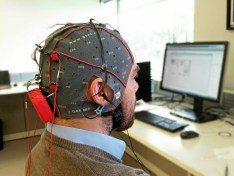
\includegraphics[width=2.25in]{images/eeg-neurotech.jpg}
%\caption*{%
%\small A neurological measurement device.\\[0.25\baselineskip]
%\tiny\color{Gray} Author: William Broek\\
%License: CC BY-SA 4.0 https://creativecommons.org/licenses/by-sa/4.0
%}
%\end{figure}
%\end{minipage}
%\end{center}
%
%% Reading:
%% https://adcare.com/massachusetts/marijuana/
%
%\end{frame}



%------------------------------------------%
% Scientific Method
%------------------------------------------%

%\begin{frame}{Our Scientific Method}
%
%\begin{enumerate}
%
%\item Experimental design: based on prior research.
%
%\vspace{1\baselineskip}
%
%\item Hypothesis generation: record!
%
%\vspace{1\baselineskip}
%
%\item Collect data.
%
%\vspace{1\baselineskip}
%
%\item Test our hypothesis.
%
%\vspace{1\baselineskip}
%
%\item Reproduce.
%
%\end{enumerate}
%
%\end{frame}


%------------------------------------------%
% Question and Hypothesis
%------------------------------------------%
\section{Question and Hypothesis}
\begin{frame}{Question and Hypothesis}

% Question of the day
\begin{center}
\begin{minipage}{.9\linewidth}
\begin{Block}{Question of the day.}

\vspace{.5\baselineskip}
\begin{itemize}

\item Can we {\bfseries curate} public Washington State pesticide data, making the data easily accessible to consumers, as a proof of concept for other states such as Oregon?


\end{itemize}

\vspace{.5\baselineskip}

\end{Block}
\end{minipage}
\end{center}

\end{frame}


%------------------------------------------%
% Takeaway
%------------------------------------------%
\section{Takeaway}
\begin{frame}{}

\begin{center}
\begin{minipage}{3.85in}

% Thank you.

\includegraphics[width=.25in]{images/prayer.png} {\Large \textbf{Thank you for coming.}}\\[-0.5\baselineskip]

\begin{center}
\begin{minipage}{\linewidth}
\begin{Block}{Insight of the Day}

\vspace{0.5\baselineskip}

\begin{itemize}

\item There are benefits that arise from {\bfseries consistency}.

\vspace{0.25\baselineskip}
\begin{itemize}

\item Consistent namespaces;

\vspace{0.25\baselineskip}

\item Consistent statistics;

\vspace{0.25\baselineskip}

\item Consistent products.

\end{itemize}

\vspace{0.5\baselineskip}

\end{itemize}

\end{Block}
\end{minipage}
\end{center}

\vfill

\end{minipage}
\end{center}

\vspace{0.5\baselineskip}
% In Saturday Morning Statistics this week, we will do just that.
What would you like to talk about next week on 4/20?

\vspace{0.5\baselineskip}

\end{frame}


%------------------------------------------%
% Fin.
%------------------------------------------%
\end{document}
